\chapter{Frequency response of the system}

\section{Introduction}

The new governing parameters (\massstiff\ and \massdamp)formulated in chapter \ref{chap:goven_para} provide a good representation of mean power output. Therefore, the next step was to identify the possibility of obtaining the frequency response through \massstiff\ and \massdamp.


\section{Linear frequency of the system}

The process was initiated by looking at the linearised galloping equation (Eq:\ref{eqn:eom_linear}). The eigenvalues of the linearised QSS model could be found in equation \ref{eqn:eigs}. The term under the square root (equation \ref{eqn:liner_freq}) of this equation can be used to express the frequency of the system provided that the term is complex. If this condition is satisfied, the imaginary component could be identified as the frequency of the system. 

\begin{equation}
\label{eqn:liner_freq}
f = \sqrt{\left[\frac{c-\frac{1}{2}\rho U\mathcal{A}a_1}{(m)}\right]^2-4\frac{k}{(m)}}.
\end{equation}



% % % % % % % % %
By substituting \cstar, \mstar\ and \ustar equation \ref{eqn:liner_freq} could be non-dimensionalised as follows:

\begin{equation}
f = \sqrt{\left[c^*\left(\frac{U}{D}\right) - \frac{1}{2}\frac{a_1}{m^*}\left(\frac{U}{D}\right)\right]^2 - 4\left(\frac{U}{D}\right)^2\frac{2\pi}{U^*}}.
\end{equation}

This can then be rewritten as
\begin{equation}
f = \sqrt{\left(\frac{U}{D}\right)^2\left(c^*-\frac{a_1}{2m^*}\right)^2 - 4\left(\frac{U}{D}\right)^2\left(\frac{2\pi}{U^*}\right)^2}.
\end{equation}
By taking the factor of $U/D$ to the left-hand side
\begin{equation}
\frac{fD}{U} = \sqrt{\left(c^*-\frac{a_1}{2m^*}\right)^2 - 4\left(\frac{2\pi}{U^*}\right)^2}.
\end{equation}
Expanding terms gives
\begin{equation}
\frac{fD}{U} = \sqrt{c^{*2} - \frac{2c^*a_1}{2m^*} + \frac{a_1^2}{4m^{*2}} - \frac{16\pi^2}{U*^2}}.
\end{equation}
Multiplying through by $m*^2$ gives
\begin{equation}
\frac{fD}{U} = \sqrt{c^{*2}m^{*2} - c^*m^*a_1 + \frac{a_1^2}{4} - \frac{16\pi^2m{*^2}}{U^{*2}}}.
\end{equation}


By substituting \massstiff\ and \massdamp\ appropriately the expression of the linear frequency reduced to   
\begin{equation}
\label{eqn:linear_freq_final}
\frac{fD}{U} = \sqrt{\Pi_2^2 - \Pi_2a_1 + \frac{a_1^2}{4} - 4\Pi_1}.
\end{equation}

Thus, from equation \ref{eqn:linear_freq_final} the non-dimensionalised linear frequency of the system could be expressed from the newly formulated terms, \massstiff\ and \massdamp.



So, by setting $f=0$, the relationship between $\Pi_1$ and $\Pi_2$ at
the limit can be found.


	% !TeX spellcheck = en_GB
	\begin{figure}[!htb]
	  \setlength{\unitlength}{\textwidth}
	
	        \begin{picture}(1,0.4)(-0.02,0)
	
	 
	      
	      \put(0.08,0.02){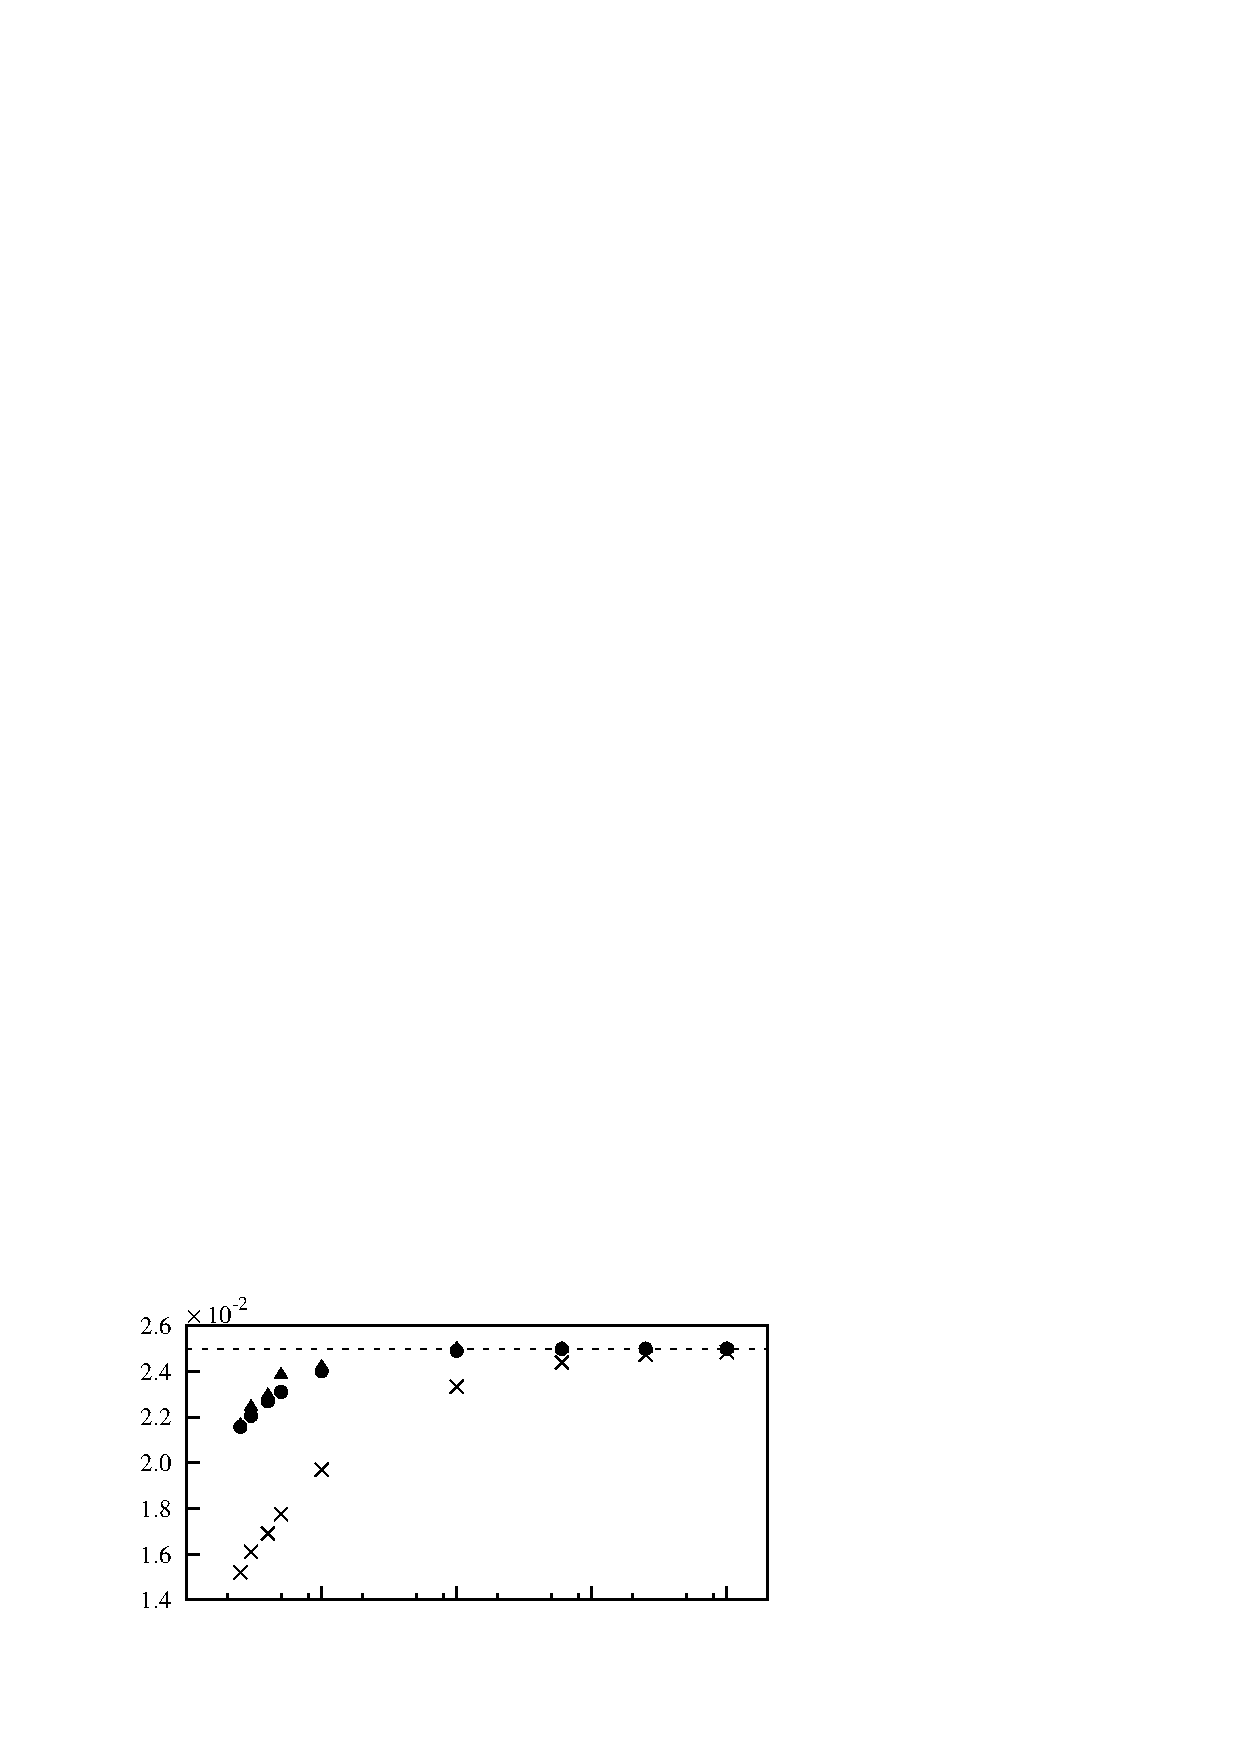
\includegraphics[width=0.75\unitlength]{{./chapter-frequnecy-response/fnp/freq015}.eps}}
	
	      \put(0.47,0.00){\massstiff}
	      
	      
	     
	       \put(0.06,0.235){$\displaystyle\frac{f_{i}}{f}$}
	      
	
	      %\put(0.095,0.218){\small(a)}
	      %\put(0.565,0.218){\small(b)}
	      
	    \end{picture}
	
	  \caption{Frequency ratio as a function of \massstiff. Frequency obtained using QSS simulations, DNS simulations and the linear frequency equation (Eq:\ref{eqn:linear_freq_final})normalised by the undamped natural frequency $f$. $f_{i}$ is the type of frequency i.e. \freqdns,\freqqss ,\freqlin. Data present $\frac{f_{lin}}{f}$ ($\bullet$), $\frac{f_{QSS}}{f}$ (\ding{115}) and $\frac{f_{DNS}}{f}$ ($\times$) at $\massdamp=0.15$, $\reynoldsnumber=200$ and undamped natural frequency, $f=0.025$. }
	    \label{fig:pi2-015-freq}
	\end{figure}
	
	 %vspace{10cm}

	% !TeX spellcheck = en_GB
	\begin{figure}[!htb]
	  \setlength{\unitlength}{\textwidth}
	
	        \begin{picture}(1,0.75)(-0.02,-0.02)
	
	 
	      
	      \put(0.08,0.03){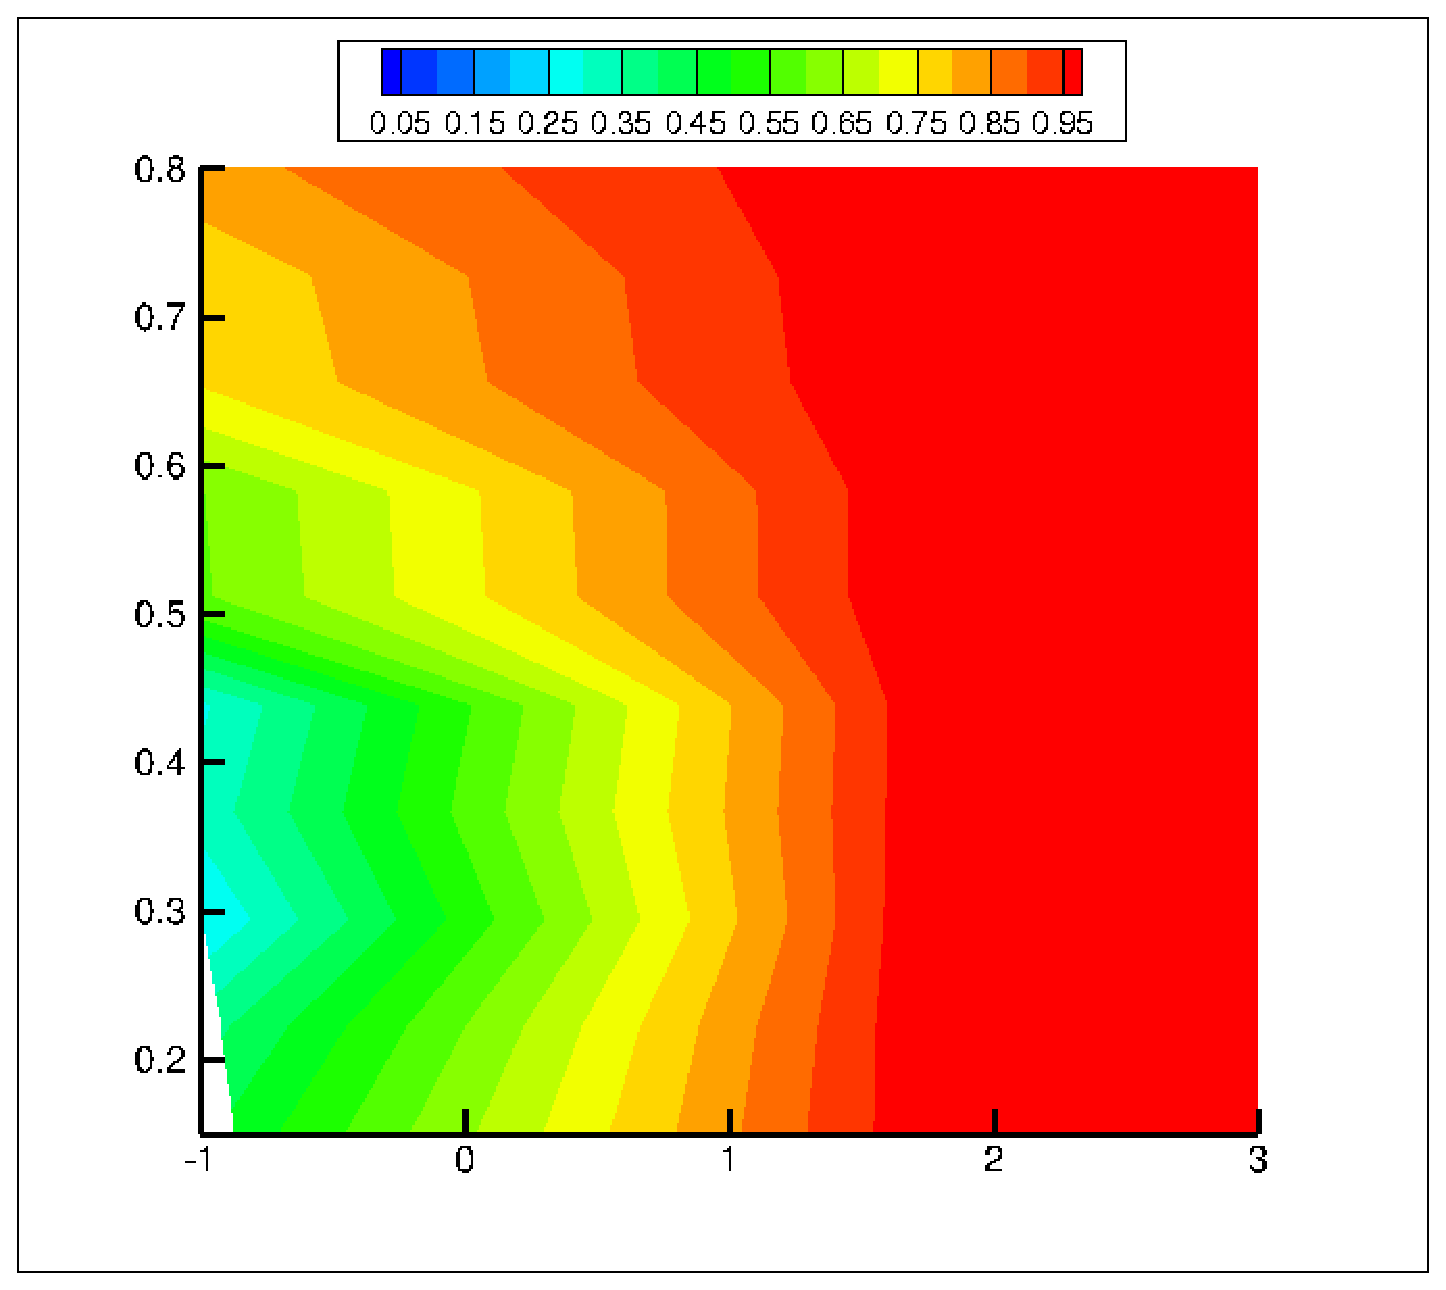
\includegraphics[width=0.75\unitlength]{./chapter-frequnecy-response/fnp/flin-fqss.eps}}
	
	      \put(0.01,0.35){\massdamp}
	      \put(0.46,0.00){$\log(\massstiff)$}
	      \put(0.18,0.65){$\frac{f_{lin}}{f_{QSS}}$}
	      
	      
	     
	       
	      
	
	      %\put(0.095,0.218){\small(a)}
	      %\put(0.565,0.218){\small(b)}
	      
	    \end{picture}
	
	  \caption{Contour plot of  $\frac{f_{lin}}{f_{QSS}}$ in $\log(\massstiff)$\ \massdamp\ space. The linear frequency \freqlin\ provides a good agreement with the frequency predicted by the quasi-steady state model beyond $\massstiff=10$}
	    \label{fig:freq-qss-linear}
	\end{figure}
	
	 %vspace{10cm}

	% !TeX spellcheck = en_GB
	\begin{figure}[!htb]
	  \setlength{\unitlength}{\textwidth}
	
	        \begin{picture}(1,0.75)(-0.02,-0.02)
	
	 
	      
	      \put(0.08,0.03){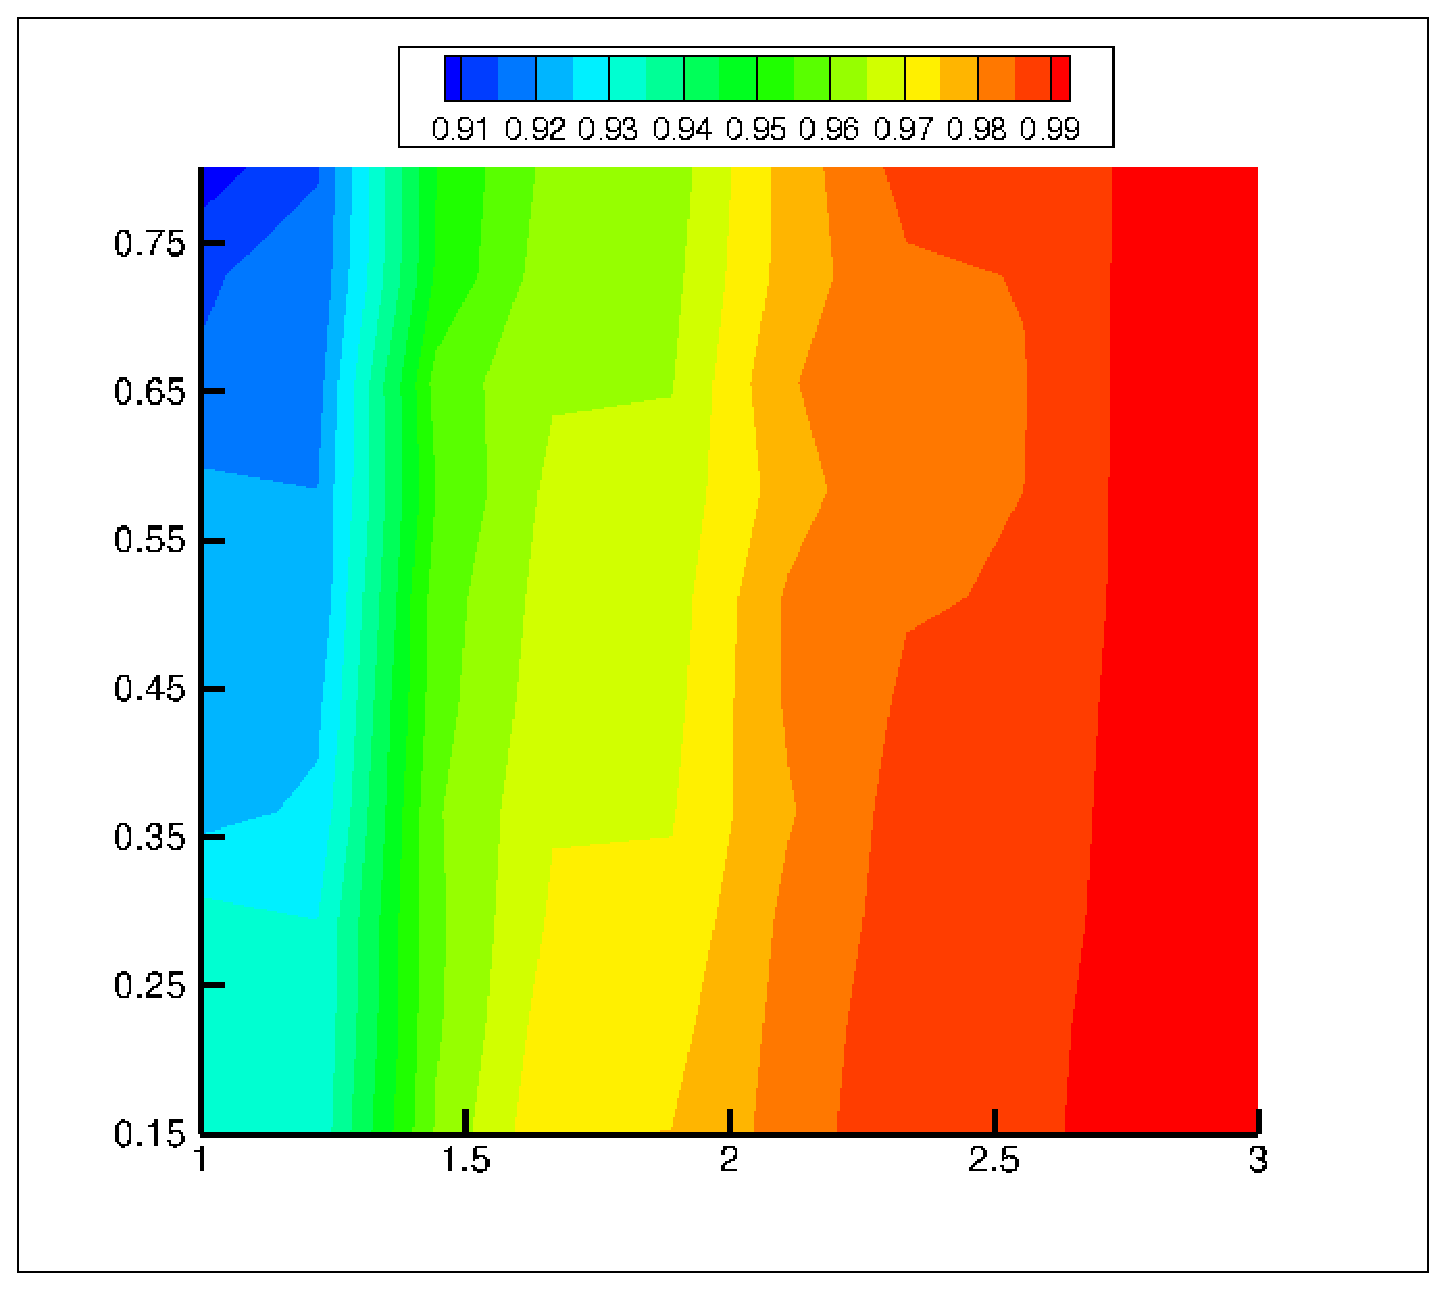
\includegraphics[width=0.75\unitlength]{./chapter-frequnecy-response/fnp/fdns-flinear.eps}}
	
	      \put(0.1,0.36){\massdamp}
	      \put(0.45,0.075){$\massstiff$}
	      \put(0.24,0.67){$\frac{f_{lin}}{f_{DNS}}$}
	      
	     
	       
	      
	
	      %\put(0.095,0.218){\small(a)}
	      %\put(0.565,0.218){\small(b)}
	      
	    \end{picture}
	
	  \caption{Contour plot of  $\frac{f_{lin}}{f_{DNS}}$ in $\massstiff$\ \massdamp\ space. The linear frequency \freqlin\ provides a good prediction of the DNS frequency over the range of \massstiff plotted here.}
	    \label{fig:feq-dns}
	\end{figure}
	
	 %vspace{10cm}

	% !TeX spellcheck = en_GB
	\begin{figure}[!htb]
	  \setlength{\unitlength}{\textwidth}
	
	        \begin{picture}(1,0.75)(-0.02,-0.02)
	
	 
	      
	      \put(0.08,0.03){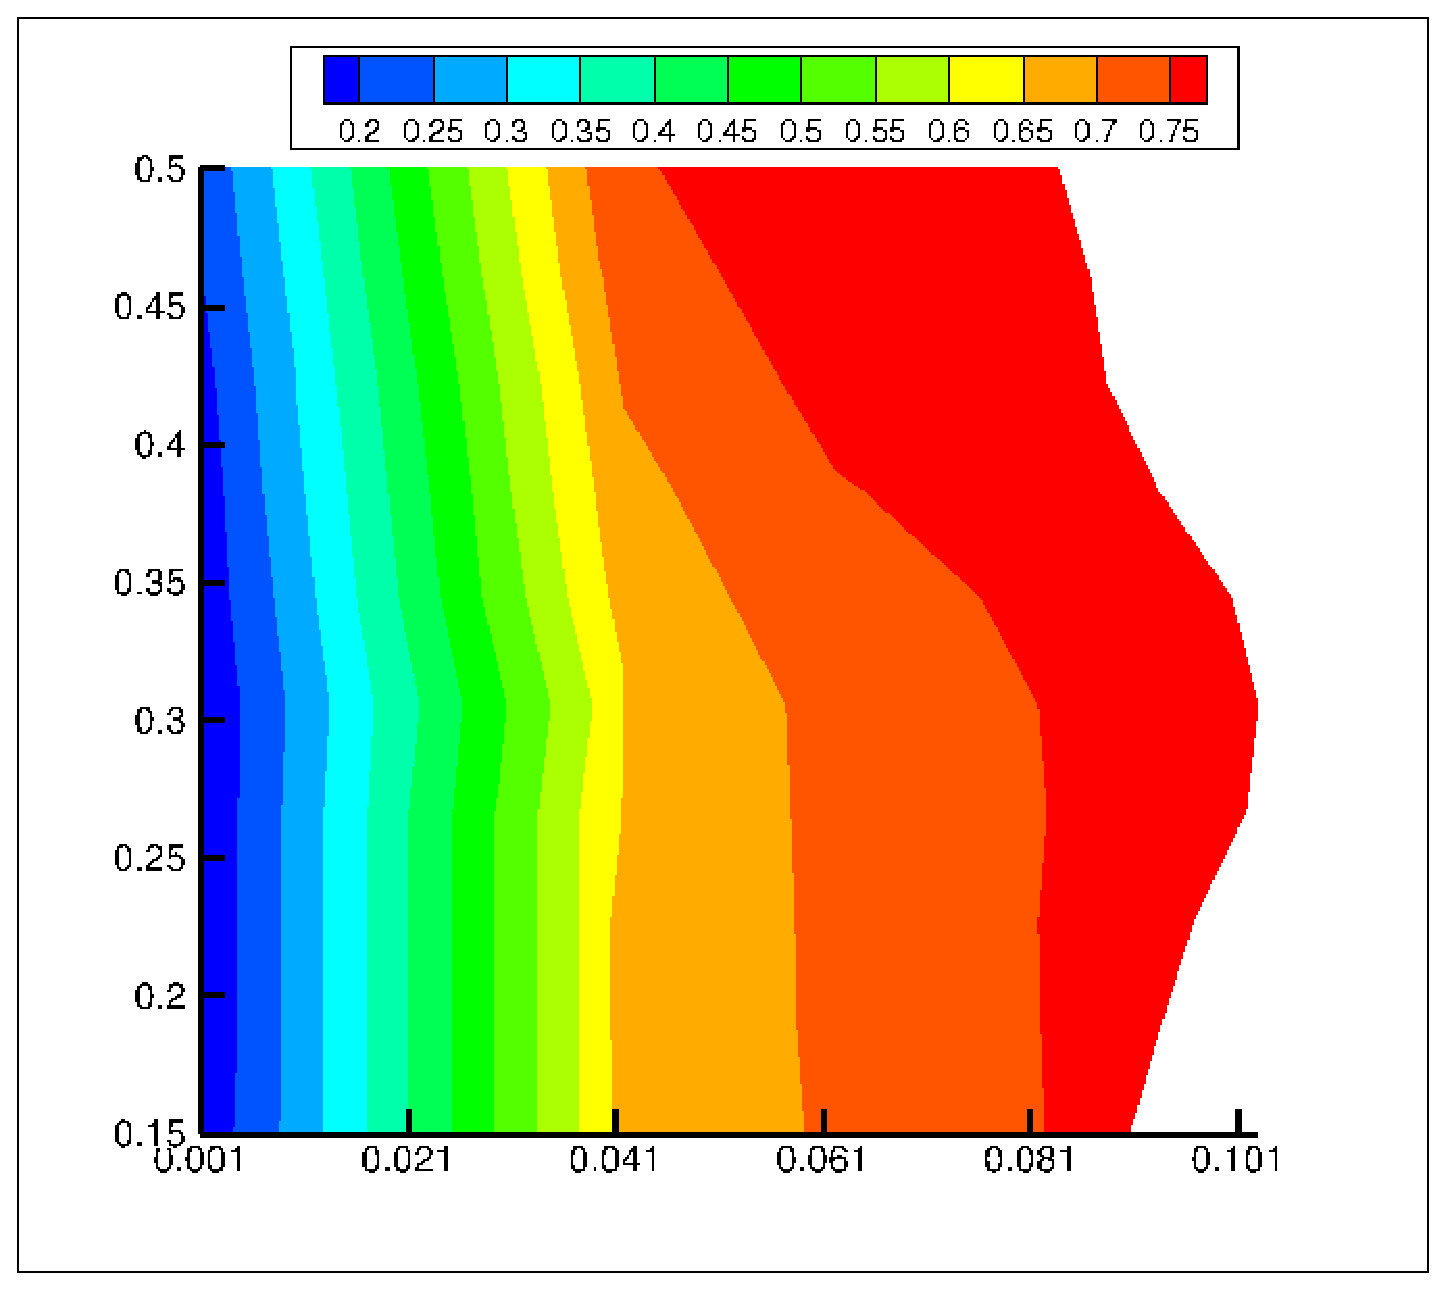
\includegraphics[width=0.75\unitlength]{./chapter-frequnecy-response/fnp/freq_non_linear.eps}}
	
	      \put(0.01,0.35){\massdamp}
	      \put(0.46,0.00){\massstiff}
	      \put(0.17,0.65){$\frac{f_{QSS}}{f}$}
	      
	     
	       
	      
	
	      %\put(0.095,0.218){\small(a)}
	      %\put(0.565,0.218){\small(b)}
	      
	    \end{picture}
	
	  \caption{Contour plot of $\frac{f_{QSS}}{f}$ in \massstiff\ \massdamp\ space, at the region where no linear frequency is predicted ($f_{lin}=0$).}
	    \label{fig:freq_non_linear}
	\end{figure}
	
	 %vspace{10cm}

%
%\section{Finding the terminal velocity of the body when no frequency
%	is predicted by equation 8}
%	
%	For very small $Pi_1$ where no frequency is predicted by equation 8,
%	we can assume that the body quickly accelerates to a velocity where
%	the lift force is blanced by the damping force. While the displacement
%	is small, the spring force is basically negligible. Also, for the
%	velocity to saturate (reach a constant value), we need only one
%	nonlinear term in the equation, and so we retain only up to the cubic
%	velocity term in the lift force to give
%	\begin{equation}
%	c\dot{y} = \frac{1}{2}\rho U^2\mathcal{A}\left[a_1\left(\frac{\dot{y}}{U}\right) + a_3\left(\frac{\dot{y}}{U}\right)^3\right].
%	\end{equation}
%	Rearranging and dividing by $\dot{y}$ gives
%	\begin{equation}
%	\left(\frac{1}{2}\rho U\mathcal{A}a_1 - c\right) + \frac{1}{2}\rho\frac{1}{U}\mathcal{A}a_3\dot{y}^2 = 0,
%	\end{equation}
%	So that the terminal velocity $\dot{y}$ is given by
%	\begin{equation}
%	\dot{y} = \pm\sqrt{-\frac{(1/2)\rho U^2\mathcal{A}a_1 - cU}{(1/2)\rho\mathcal{A}a_3}}.
%	\end{equation}
%	This can be written as
%	\begin{equation}
%	\dot{y} = \pm\sqrt{U^2\frac{a_1}{a_3} - U^2\frac{c}{(1/2)\rho U\mathcal{A}a_3}}
%	\end{equation}
%	or
%	\begin{equation}
%	\frac{\dot{y}}{U} = \pm\sqrt{\frac{a_1}{a_3} - \frac{c}{(1/2)\rho U\mathcal{A}a_3}}.
%	\end{equation}
%	
%	Finally, the definition of $\Pi_2$ can be substituted into the last term to give
%	\begin{equation}
%	\frac{\dot{y}}{U} = \pm\sqrt{\frac{1}{a_3}(a_1 - 2\Pi_2)},
%	\end{equation}
%	hence the terminal, or maximum velocity is a function of $\Pi_2$ only.




